\documentclass[tikz,border=5pt]{standalone}
\usepackage[UTF8]{ctex}
\usepackage{amsmath,amssymb}
\usetikzlibrary{arrows.meta,calc}
\definecolor{ink}{HTML}{243447}\definecolor{blue}{HTML}{2765A2}
\definecolor{green}{HTML}{3F7D5B}\definecolor{red}{HTML}{B74739}
\tikzset{body/.style={draw=ink,thick},vec/.style={draw=blue,thick,-{Latex}},
guide/.style={gray!60,dashed},dim/.style={ink,{Latex}-{Latex}},
line cap=round,line join=round}
\newcommand{\patternlayer}[2]{
\pgfmathsetmacro{\Rlayer}{#1/pow(3,#2/2)}
\foreach\k in{0,...,5}{
\pgfmathsetmacro{\ang}{60*\k+30*#2}
\filldraw[fill=blue!17,draw=ink,line width=.45pt]
(\ang:\Rlayer)--({\ang+30}:{\Rlayer/sqrt(3)})
--({\ang-30}:{\Rlayer/sqrt(3)})--cycle;}}
\begin{document}
\begin{tikzpicture}
\foreach\x/\n in{0/1,4/2,8/3}{
\begin{scope}[shift={(\x,0)}]
\draw[body](0:1.7)--(60:1.7)--(120:1.7)--(180:1.7)--(240:1.7)--(300:1.7)--cycle;
\pgfmathtruncatemacro{\lastlayer}{\n-1}
\foreach\j in{0,...,\lastlayer}\patternlayer{1.7}{\j}
\fill[ink](0,0)circle(.025);
\node at(0,-2.1){$\n$层};
\end{scope}}
\node[below left]at(0,0){$O$};
\draw[dim](0,0)--(1.7,0)node[midway,above]{$r$};
\end{tikzpicture}
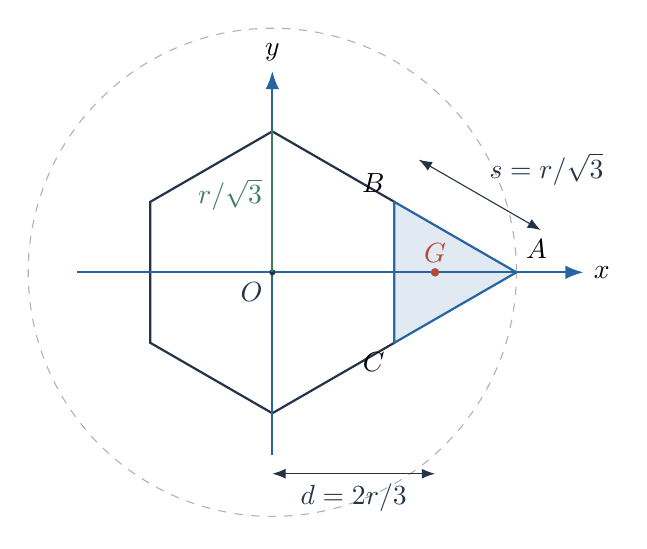
\begin{tikzpicture}[scale=1.55]
\draw[guide](0,0)circle(2);
\draw[body](30:{2/sqrt(3)})--(90:{2/sqrt(3)})
--(150:{2/sqrt(3)})--(210:{2/sqrt(3)})
--(270:{2/sqrt(3)})--(330:{2/sqrt(3)})--cycle;
\filldraw[fill=blue!14,draw=blue,thick](2,0)--(1,{1/sqrt(3)})--(1,{-1/sqrt(3)})--cycle;
\draw[vec](-1.6,0)--(2.55,0)node[right]{$x$};
\draw[vec](0,-1.5)--(0,1.65)node[above]{$y$};
\fill[ink](0,0)circle(.025)node[below left]{$O$};
\fill[red](1.3333,0)circle(.035)node[above]{$G$};
\node[above right]at(2,.03){$A$};
\node[above left]at(1,{1/sqrt(3)}){$B$};
\node[below left]at(1,{-1/sqrt(3)}){$C$};
\draw[dim](0,-1.65)--(1.3333,-1.65)node[midway,below]{$d=2r/3$};
\draw[green,thick](0,0)--(90:{2/sqrt(3)})node[pos=.55,left]{$r/\sqrt3$};
\draw[dim](1.2,.923)--(2.2,.346)node[midway,above right]{$s=r/\sqrt3$};
\end{tikzpicture}
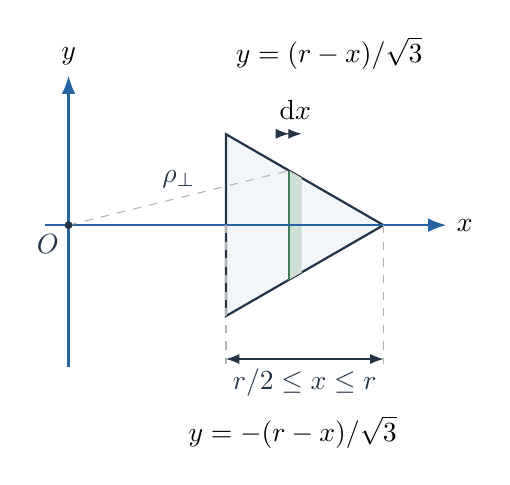
\begin{tikzpicture}[x=2cm,y=2cm]
\filldraw[fill=blue!6,draw=ink,thick](2,0)--(1,{1/sqrt(3)})--(1,{-1/sqrt(3)})--cycle;
\fill[green!25](1.4,{.6/sqrt(3)})--(1.48,{.52/sqrt(3)})
--(1.48,{-.52/sqrt(3)})--(1.4,{-.6/sqrt(3)})--cycle;
\draw[green,thick](1.4,{-.6/sqrt(3)})--(1.4,{.6/sqrt(3)});
\draw[vec](-.15,0)--(2.4,0)node[right]{$x$};
\draw[vec](0,-.9)--(0,.95)node[above]{$y$};
\draw[guide](1,0)--(1,-.88);
\draw[guide](2,0)--(2,-.88);
\draw[dim](1,-.85)--(2,-.85)node[midway,below]{$r/2\le x\le r$};
\node[above right]at(1,.93){$y=(r-x)/\sqrt3$};
\node[below right]at(.7,-1.15){$y=-(r-x)/\sqrt3$};
\draw[dim](1.4,.58)--(1.48,.58);
\node[above]at(1.44,.61){$\mathrm dx$};
\draw[guide](0,0)--(1.4,{.6/sqrt(3)})node[midway,above,text=ink]{$\rho_\perp$};
\fill[ink](0,0)circle(.025)node[below left]{$O$};
\end{tikzpicture}
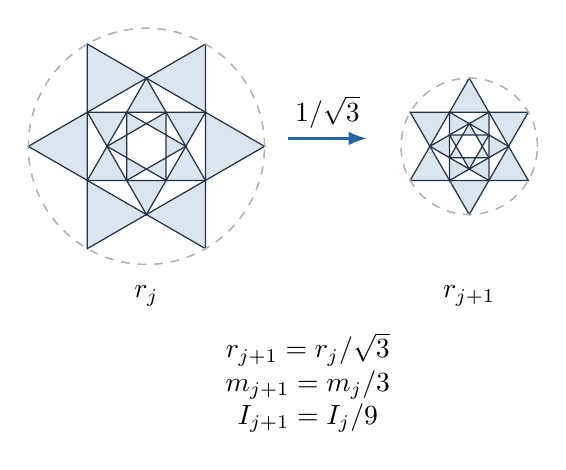
\begin{tikzpicture}
\begin{scope}
\foreach\j in{0,1,2}\patternlayer{1.5}{\j}
\draw[guide](0,0)circle(1.5);
\node at(0,-1.9){$r_j$};
\end{scope}
\begin{scope}[shift={(4.1,0)}]
\foreach\j in{1,2,3}\patternlayer{1.5}{\j}
\draw[guide](0,0)circle(.866025);
\node at(0,-1.9){$r_{j+1}$};
\end{scope}
\draw[vec](1.8,.1)--(2.8,.1)node[midway,above]{$1/\sqrt3$};
\node[align=center]at(2.05,-3.0){$r_{j+1}=r_j/\sqrt3$\\$m_{j+1}=m_j/3$\\$I_{j+1}=I_j/9$};
\end{tikzpicture}
\end{document}
